Bei der Erforschung des hei{\ss}en und dichten Mediums und der Suche nach dem QGP spielt das Phasendiagramm stark wechselwirkender Materie eine wichtige Rolle.
\grqq{}Wie sieht der Phasenu\"ubergang aus?\grqq{}, oder \grqq{}Wann findet der Phasen\"ubergang statt?\grqq{} sind beispielhaft zwei Fragen, die es zu beantworten gilt.
\begin{figure}[tbp]
\centering
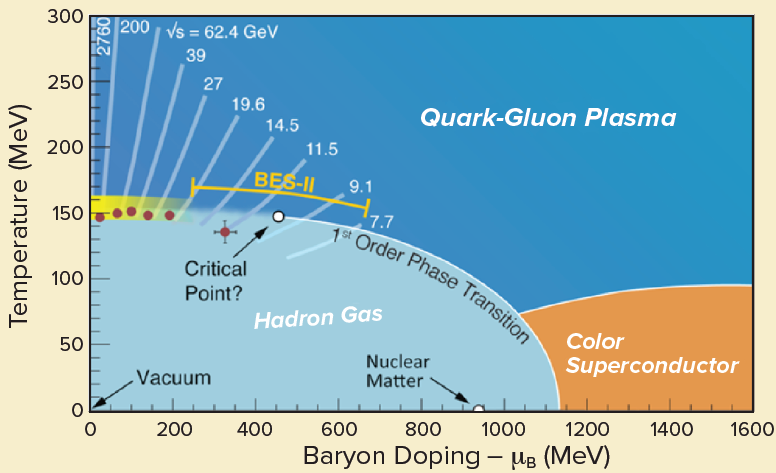
\includegraphics[width=.7\linewidth]{QGPPhaseDiagram.png}
\caption{Phasendiagramm des Quark-Gluon-Plasmas in Abh\"angigkeit der Baryonendichte $\mu_{\text{B}}$ und der Temperatur $T$.
[https://arxiv.org/abs/1609.03104]}
\label{fig:QGPPhase}
\end{figure}
Abbildung \ref{fig:QGPPhase} skizziert ein Phasendiagramm stark wechselwirkender Materie. In der Abbildung befinden sich au{\ss}erdem eingezeichnet verschiedene Schwerpunktsenergieen $\sqrt{s}$.
Um ein hei{\ss}es und dichtes Medium untersuchen zu k\"onne, muss dieses zun\"achst einmal im Labor erzeugt werden.
Wie im vorherigen Abschnitt beschrieben, ist zur Erzeugung eines solchen hei{\ss}en und dichten Zustands die Kollision zweier hochenergetischen Atomkerne n\"otig.
F\"ur Referenzmessungen werden aber auch unter anderem Proton-Proton-Kollisionen gemessen.
Solche Kollisionen werden in sogenannten Colliderexperimenten durchgef\"uhrt.
Ein solches Colliderexperiment wird am CERN betrieben.
Das CERN ist Europas gr\"o{\ss}tes Institut zur Untersuchung im Bereich der (Elementar)Teilchenphysik.
Am CERN befindet sich das, nach aktuellem Stand, gr\"o{\ss}te Colliderexperiment weltweit.

Bevor hochenergetische Kerne oder Teilchen zum Kollidieren gebracht werden m\"ssen die zun\"achst nicht relativistischen Kerne oder Teilchen beschleunigt werden.
Dies geschieht in sogenannten Beschleunigerringen, der gr\"o{\ss}te Beschleunigerring ist der sogenannte LHC.
Die Kollisionen werden an vier Punkten im LHC provoziert.
An allen vier Stellen befinden sich umfangreiche Detektorkomplexe, wie etwa der ALICE Detektor.
Im folgenden Abschnitt wird das ALICE Experiment genauer beschrieben.